\documentclass{standalone}
\usepackage{tikz}
\usepackage{pgfplots}
\pgfplotsset{width=32cm,height=18cm,compat=1.3}
\pgfplotsset{every tick label/.append style={font=\Huge}}
\usepackage{filecontents}
\usepgfplotslibrary{fillbetween}

\usetikzlibrary{patterns}

\definecolor{citrine}{rgb}{0.89, 0.82, 0.04}

\begin{document}
	\centering
		\vspace{1.5em}
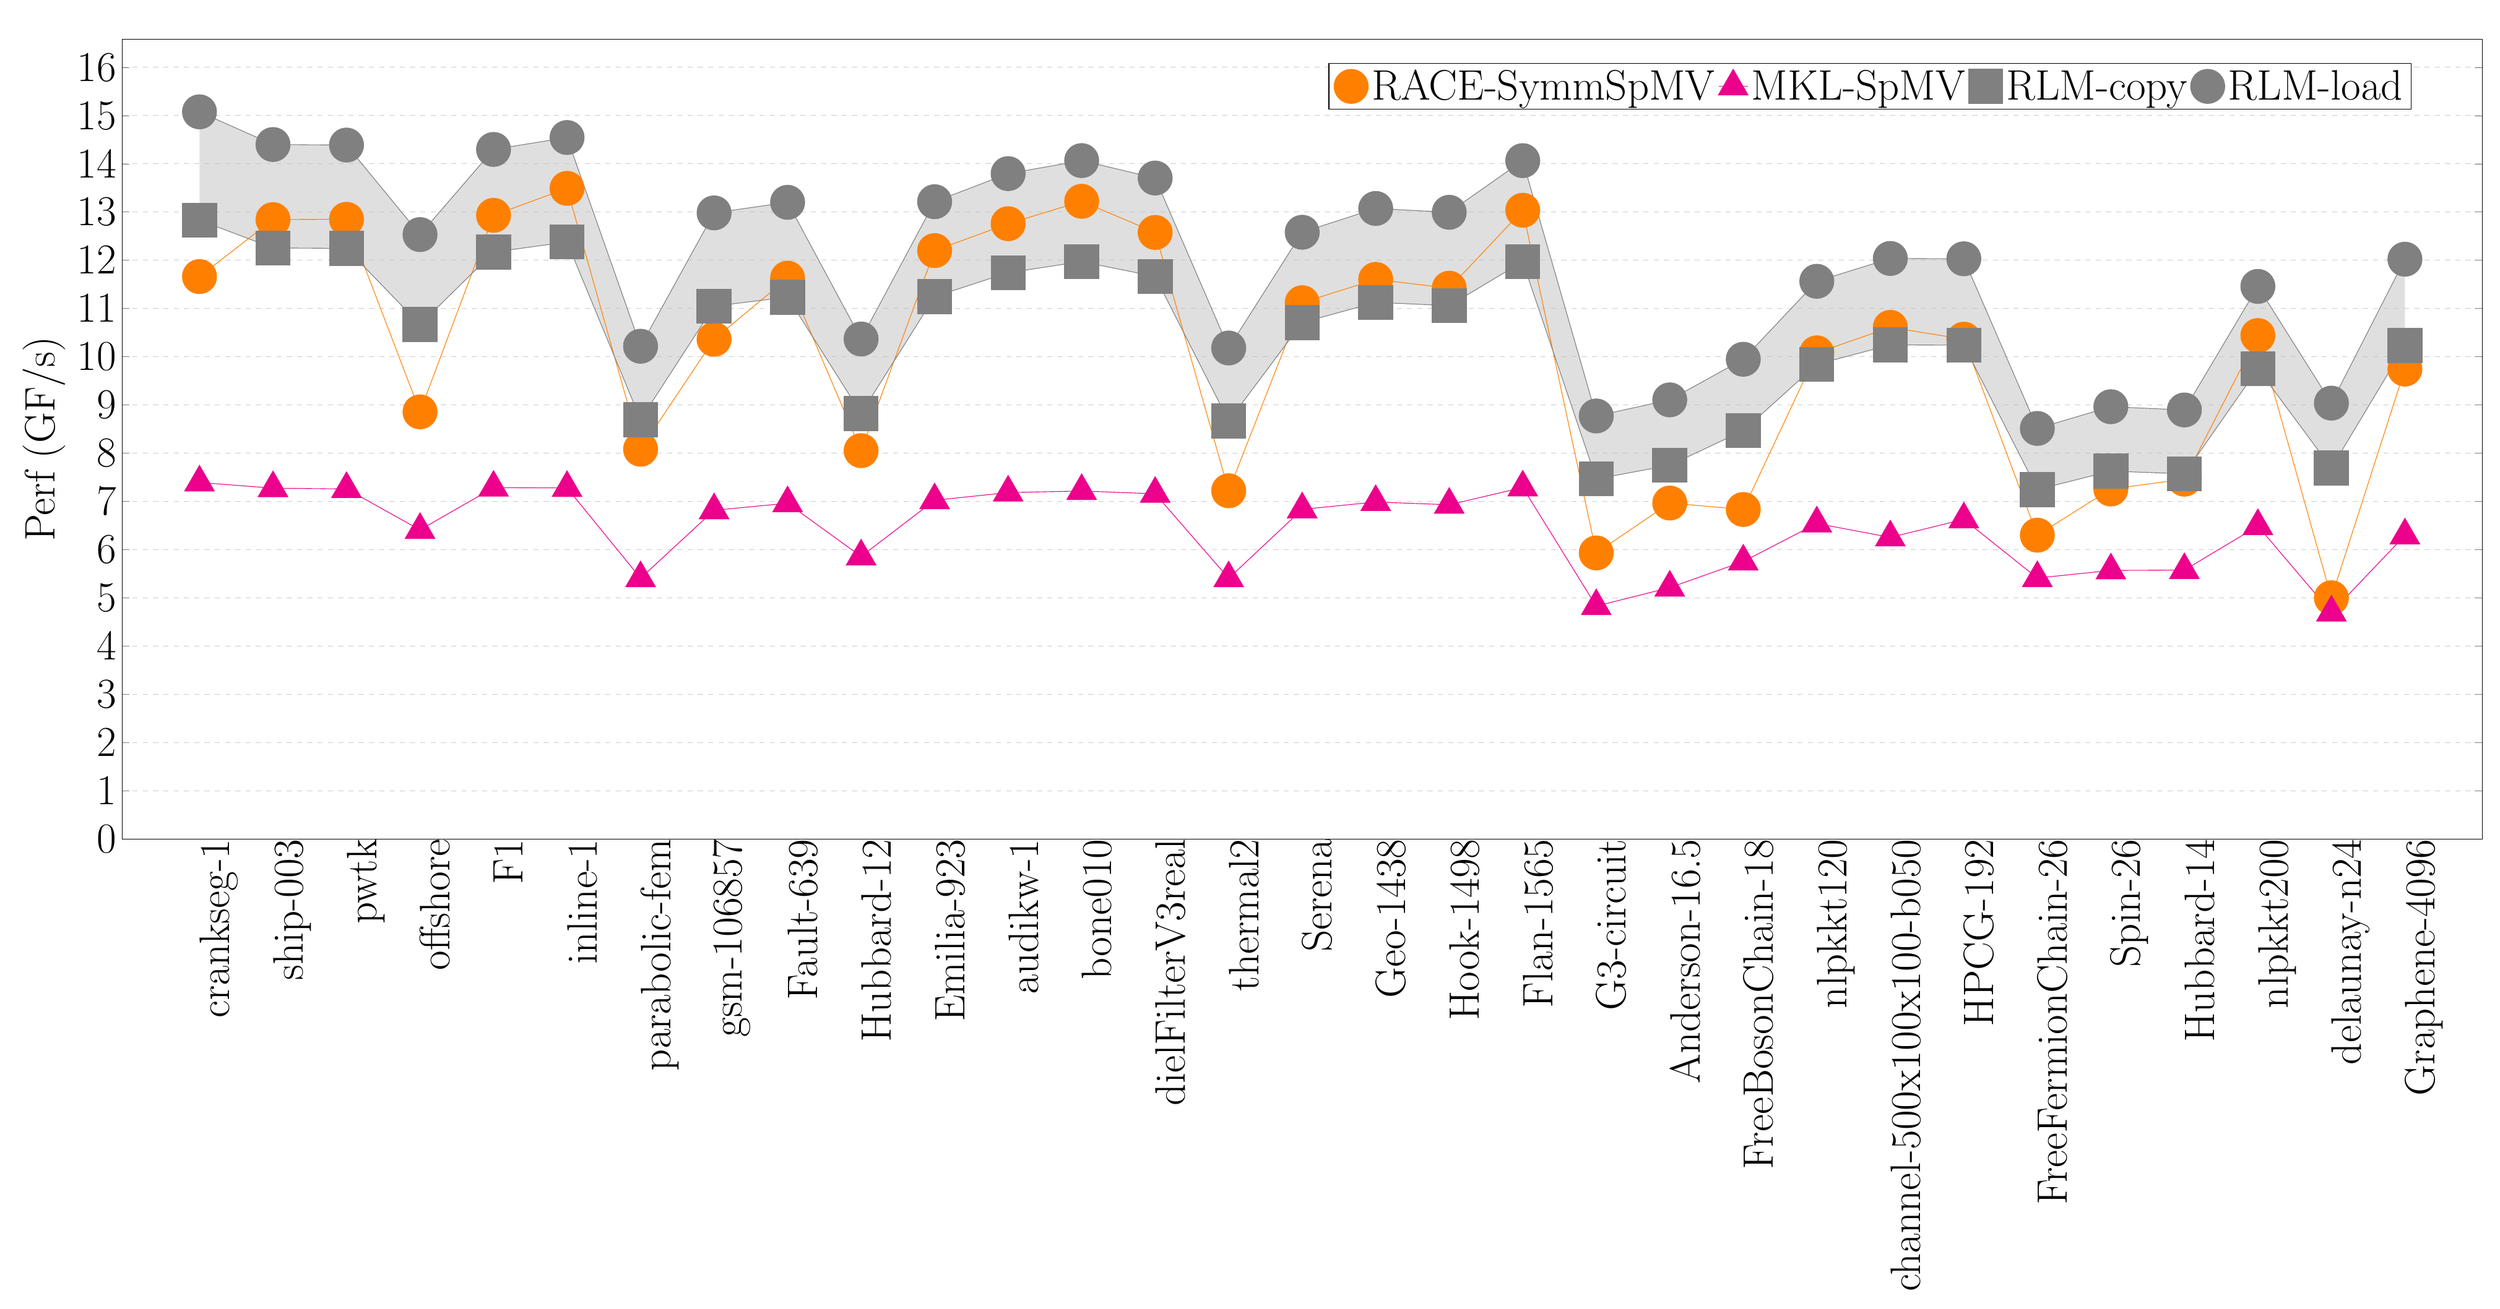
\begin{tikzpicture}
		%	\node at (13.25,15) {\LARGE{}};
			\begin{axis}[
		%	xmin=0.25, xmax=7.25,
			ymin=0, %ymax=3.25,
			xtick={1, 2, 3, 4, 5, 6, 7, 8, 9, 10, 11, 12, 13, 14, 15, 16, 17, 18, 19, 20, 21, 22, 23, 24, 25, 26, 27, 28, 29, 30, 31},
		%	ytick={0,0.5,1,1.5,2,2.5,3},
			xticklabels={crankseg-1, ship-003, pwtk, offshore, F1, inline-1, parabolic-fem, gsm-106857, Fault-639, Hubbard-12, Emilia-923, audikw-1, bone010, dielFilterV3real, thermal2, Serena, Geo-1438, Hook-1498, Flan-1565, G3-circuit, Anderson-16.5, FreeBosonChain-18, nlpkkt120, channel-500x100x100-b050, HPCG-192, FreeFermionChain-26, Spin-26, Hubbard-14, nlpkkt200, delaunay-n24, Graphene-4096},
			width  = 50cm,
			height = 18cm,
			major x tick style = transparent,
			%	minor ytick={1, 5, 10, 15, 20, 25, 30 ,35,40},
			grid = minor,	
			%add_bar_commands
			ymajorgrids = true,
			grid style={dashed, gray!40},
			ylabel = {\Huge{Perf (GF/s)}},
		%	symbolic x coords={Graphene-2048-2048, Graphene-4096-4096, Spin-24-24-24},
			x tick label style={rotate=90, anchor=north east, inner sep=0mm, font={\Huge}},
			tick label style={font={\Huge}},
			scaled y ticks = false,
			enlarge x limits=0.035,
			legend cell align=left,
			legend style={font=\Huge},
			legend columns=-1,
			legend style={
				%at={(1,1.05)},
				%anchor=south east,
				%column sep=1ex,
				legend pos=north east
			},
			%spl_legend_code
			title= {\Huge\scalebox{1.5}{{}}}
			]

\addplot[name path=RACE-SymmSpMV, mark=*, mark size=10pt, mark options={orange}, draw=orange ] plot coordinates{(1,11.661889) (2,12.843037) (3,12.849712) (4,8.856331) (5,12.932172) (6,13.490943) (7,8.080436) (8,10.361301) (9,11.629001) (10,8.051711) (11,12.200132) (12,12.757774) (13,13.222356) (14,12.576653) (15,7.219646) (16,11.119455) (17,11.603120) (18,11.420717) (19,13.037058) (20,5.930575) (21,6.965104) (22,6.831253) (23,10.080070) (24,10.609130) (25,10.363803) (26,6.298190) (27,7.255795) (28,7.459718) (29,10.439037) (30,4.999955) (31,9.742837)};
\addplot[name path=MKL-SpMV, mark=triangle*, mark size=10pt, mark options={magenta}, draw=magenta ] plot coordinates{(1,7.391667) (2,7.273372) (3,7.256906) (4,6.408492) (5,7.284015) (6,7.278270) (7,5.406702) (8,6.814587) (9,6.960603) (10,5.857076) (11,7.022496) (12,7.181654) (13,7.214559) (14,7.156261) (15,5.405101) (16,6.834216) (17,6.986155) (18,6.929315) (19,7.287457) (20,4.826937) (21,5.211025) (22,5.752017) (23,6.541114) (24,6.252774) (25,6.626783) (26,5.409494) (27,5.567883) (28,5.574583) (29,6.487564) (30,4.693660) (31,6.293212)};
\addplot[name path=RLM-copy, mark=square*, mark size=10pt, mark options={gray}, draw=gray ] plot coordinates{(1,12.832208112931099) (2,12.255316183172415) (3,12.24579212158689) (4,10.66557267698624) (5,12.169045654359836) (6,12.379032966847529) (7,8.695266491316243) (8,11.04894638481779) (9,11.235375160606813) (10,8.823041190350098) (11,11.246044953764729) (12,11.741961159697489) (13,11.97178228869749) (14,11.663676576430914) (15,8.664268964057458) (16,10.706817789946504) (17,11.126959076176266) (18,11.059164805349113) (19,11.971024715057927) (20,7.4643757233720995) (21,7.748499212558767) (22,8.465222498643278) (23,9.841487979651877) (24,10.24454198231261) (25,10.238860356373173) (26,7.244496068452896) (27,7.627736943253068) (28,7.570245815299977) (29,9.751108262734487) (30,7.690981692206367) (31,10.2313409263867)};
\addplot[name path=RLM-load, mark=*, mark size=10pt, mark options={gray}, draw=gray ] plot coordinates{(1,15.07784453269404) (2,14.399996515227588) (3,14.388805742864594) (4,12.532047895458833) (5,14.298628643872807) (6,14.545363736045847) (7,10.216938127296586) (8,12.9825120021609) (9,13.201565813713005) (10,10.367073398661365) (11,13.214102820673556) (12,13.79680436264455) (13,14.066844189219552) (14,13.704819977306325) (15,10.180516032767512) (16,12.580510903187141) (17,13.074176914507113) (18,12.994518646285208) (19,14.065954040193065) (20,8.770641474962217) (21,9.104486574756551) (22,9.946636435905852) (23,11.563748376090956) (24,12.037336829217317) (25,12.03066091873848) (26,8.512282880432153) (27,8.962590908322355) (28,8.895038832977471) (29,11.457552208713022) (30,9.036903488342482) (31,12.021825588504374)};
\addplot[fill=lightgray,opacity=0.5]
fill between[of= RLM-copy and RLM-load];
	%addplot cmd

	\legend{RACE-SymmSpMV, MKL-SpMV, RLM-copy, RLM-load}

	\end{axis}			
\end{tikzpicture}

\end{document}

